\documentclass[a4paper,norsk, 10pt]{article}
\usepackage[utf8]{inputenc}
\usepackage{verbatim}
\usepackage{listings}
\usepackage{graphicx}
\usepackage[norsk]{babel}
\usepackage{a4wide}
\usepackage{color}
\usepackage{amsmath}
\usepackage{float}
\usepackage{amssymb}
\usepackage[dvips]{epsfig}
\usepackage[toc,page]{appendix}
\usepackage[T1]{fontenc}
\usepackage{cite} % [2,3,4] --> [2--4]
\usepackage{shadow}
\usepackage{hyperref}
\usepackage{titling}
\usepackage{marvosym }
\usepackage{subcaption}
\usepackage[noabbrev]{cleveref}
\usepackage{cite}


\setlength{\droptitle}{-10em}   % This is your set screw

\setcounter{tocdepth}{2}

\lstset{language=c++}
\lstset{alsolanguage=[90]Fortran}
\lstset{alsolanguage=Python}
\lstset{basicstyle=\small}
\lstset{backgroundcolor=\color{white}}
\lstset{frame=single}
\lstset{stringstyle=\ttfamily}
\lstset{keywordstyle=\color{red}\bfseries}
\lstset{commentstyle=\itshape\color{blue}}
\lstset{showspaces=false}
\lstset{showstringspaces=false}
\lstset{showtabs=false}
\lstset{breaklines}
\title{FYS2140 Oblig 2}
\author{Daniel Heinesen, daniehei}
\begin{document}
\maketitle

\section*{3.3)}

\subsection*{a)}

Energien som frigitt av atomet er gitt som $E = E_1-E_2$. Dette energien blir til et foton, men noe av den blir også gitt til atomet i forme av kinetisk energi. Vi antar at den kinetiske energien atomet får er ikke-relativistisk

$$
E_k = \frac{p^2}{2m}
$$ 

Vi trenger da å finne bevegelsesmengden. Vi antar at atomet stod stille før emitteringen. Det emitterte fotonet har $p_{\gamma} = \frac{h\nu}{c}$. Så

$$
p_k + p_{\gamma} = 0
$$

$$
p_k = -p_{\gamma} = -\frac{h\nu}{c}
$$

vi for da at den kinetiske energien til atomet blir

$$
E_k = \frac{h^2\nu^2}{2Mc^2}
$$

Vi vet da at den totale energien etter emitteringen er

$$
E = h\nu + \frac{h^2\nu^2}{2Mc^2} = E_1 - E_2
$$

$$
\Rightarrow h\nu = E_1 - E_2 - \frac{h^2\nu^2}{2mc^2}
$$

Dette gir oss at 

\begin{equation}
\Delta E = \frac{h^2\nu^2}{2Mc^2}
\label{eq:dE}
\end{equation}

\subsection*{b)}

Nå har vi et atom med masse $M$ og et foton med energi $h\nu$ og bevegelsemengde $\frac{h\nu}{c}$. Atomet har også energi $E_1$. Når fotonet treffer atomet får det energi $E_2$. I tillegg får det en kinetisk energi $\Delta E$. Så

$$
h\nu + E_1 = E_2 +\Delta E
$$

Vi antar også at atomet stod stille får sammenstøtet, og får bevegelsemengden $p_k$ etter, mens fotonet vil bli borte og ikke lenger ha noe bevegelsemengde. Derfor

$$
p_k + 0 = \frac{h\nu}{c} + 0
$$

Dette gir oss akkurat de samme uttrykket som i a), og vi får igjen at

$$
\Delta E = \frac{h^2\nu^2}{2Mc^2}
$$

\subsection*{c)}

\textbf{FYLL INN HER}

\section*{3.5)}

Vi har potensialet 

\begin{equation}
V(r) = V_0\left(\frac{r}{a}\right)^k
\label{eq:pot}
\end{equation}

og kvantifiseringsbetingelsen

$$
L = n\hbar
$$

Siden $L = mvr$, kan betingelsen gi oss et uttrykk for $r$

\begin{equation}
r = \frac{n\hbar}{mv}
\label{eq:r}
\end{equation}

Vi trenger nå å gjøre noe med potensialet. Vi trenger å få et uttrykk for kraften, noe vi vet er gitt ved

$$
F = -\frac{dV(r)}{dt} = -\frac{V_0k}{a^k}r^{k-1}
$$

Om partikkelen skal gå i bane rundt dette potentialet vet vi også at

$$
F = \frac{mv^2}{r} = \frac{V_0k}{a^k}r^{k-1}
$$

Om vi løser dette for hastigheten finner vi at 

\begin{equation}
v^2 = -\frac{V_0kr}{ma^k}r^{k-1} = \frac{V_0k}{ma^k}r^{k}
\label{eq:v2}
\end{equation}

Den totale energien til partikkelen er da gitt ved

\begin{equation}
E = \frac{1}{2}mv^2 + V(r) = \frac{V_0k}{2a^k}r^{k} + V_0\left(\frac{r}{a}\right)^k = \frac{V_0(k+2)r^k}{2a^k}
\label{eq:E}
\end{equation}

Vi ønsker å å fjerne avhengigheten på $r$. Vi kan gjøre dette ved å sette inn uttrykket for hastigheten \ref{eq:v2} inn i uttrykket for $r$\ref{eq:r}

$$
r(n) = \left(\frac{\hbar^2 a^k}{mV_0k}n^2\right)^{\frac{1}{k+2}}
$$

Setter vi nå dette inn i energien finner vi at 

\begin{equation}
E(n;k) = \frac{V_0(k+2)}{2a^k}\left(\frac{\hbar^2 a^k}{mV_0k}n^2\right)^{\frac{k}{k+2}}
\end{equation}

Vi kan nå sjekke om dette blir Bohrs formal om $k = -1$:

$$
E(n;-1) = \frac{V_0(-1+2)}{2a^-1}\left(\frac{\hbar^2 a^-1}{mV_0(-1)}n^2\right)^{\frac{-1}{-1+2}} = -(V_0a)^2\frac{m}{2\hbar}\frac{1}{n^2}
$$

Om vi setter $(V_0a)^2 = k_e^2e^4$ får vi Bohrs formel.\\

Vi kan nå ser på plottet av $V(r)$ for store verdier av $k$

\begin{figure}[H]
\centering
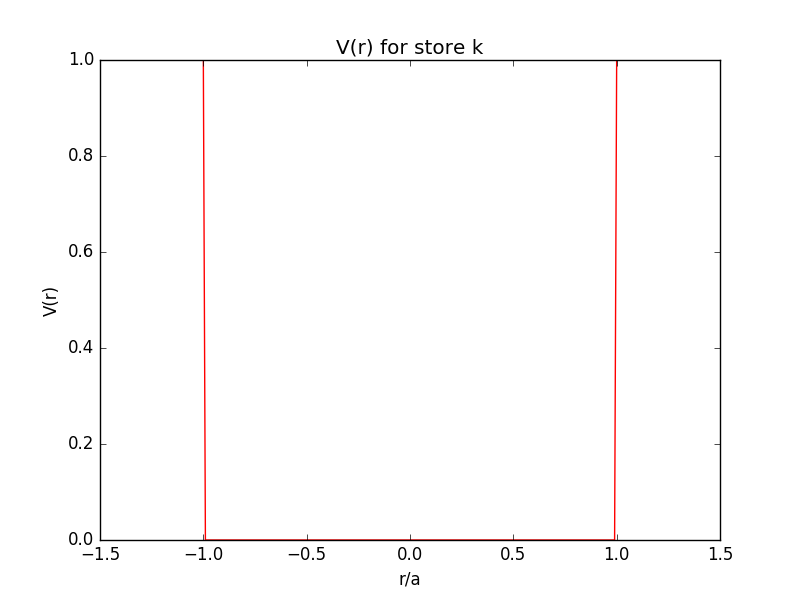
\includegraphics[scale=0.3]{vr.png}
\caption{Vi kan se at ved $\pm 1$ går $V(r)$ mot uendelig.}
\end{figure}

Vi $V(r)$ divergerer ved $ \frac{r}{a} = \pm 1$ når $k$ blir stor(går mot uendelig). Vi får da et såkalt brønnpotensial.

\section*{4.2)}

\subsection*{a)}
Vi vet at de Broglies bølgelengde er gitt ved

\begin{equation}
\lambda = \frac{h}{p}
\label{deBrog}
\end{equation}

Vi trenger derfor et uttrykk bevegelsemengden. Til dette kan vi bruke energien

$$
E = \sqrt{p^2c^2 + m_0^2c^4}
$$

$$
\Rightarrow p = \sqrt{\left(\frac{E}{c}\right)^2 -m_0c^2}
$$

Den relativistiske energien kan også skrives som

$$
E = KE + m_0c^2
$$

Partikkelen akselereres i et elektrisk feil, noe som gir den kinetiske energien $KE = eV$. Så setter vi energien $E = eV + m_0c^2$ inn i utrykket for $p$ finner vi

$$
p = \sqrt{\left(\frac{eV + m_0c^2}{c}\right)^2 -m_0c^2}
$$

$$
= \sqrt{\frac{e^2V^2 +2eV_0m_0^2 + m_0^2c^4}{c^2} - m_0c^2}
$$

$$
= \sqrt{\left(\frac{eV}{c}\right)^2 + 2eV_0m_0}
$$

$$
= \sqrt{2eV_0m_0}\left(1+\frac{eV}{2m_0c^2}\right)^{1/2}
$$

Vi kan nå sette dette inn i \ref{deBrog}, og vi får da bølgelengden

\begin{equation}
\lambda = \frac{h}{p} = \frac{h}{\sqrt{2eV_0m_0}}\left(1+\frac{eV}{2m_0c^2}\right)^{-1/2}
\end{equation}

\subsection*{b)}
Vi brukte at $eV$ for $KE$ når vi utledet uttrykket over. Om vi setter $KE$ tilbake, finner vi at 

$$
\lambda = \frac{h}{p} = \frac{h}{\sqrt{2KEm_0}}\left(1+\frac{KE}{2m_0c^2}\right)^{-1/2}
$$

I den ikke-relativistiske grensen er $KE = \frac{1}{2}m_0v^2$. Setter vi dette inn får vi

$$
\lambda = \frac{h}{p} = \frac{h}{\sqrt{m_0^2v^2}}\left(1+\frac{v^2}{4c^2}\right)^{-1/2}
$$

Siden $c>>v$ så er $\frac{v}{c}\approx 0$

$$
\lambda = \frac{h}{\sqrt{m_0v^2}}(1+0) = \frac{h}{m_0v}
$$

Noe som stemmer godt med at 

$$
\lambda = \frac{h}{p}
$$

\subsection*{c)}

Vi skal nå regne ut \ref{deBrog} med en relativistisk bevegelsemengde $p = \gamma m_0v$, der 

$$
\gamma = \frac{1}{\sqrt{1-\frac{v}{c}}} = \frac{1}{\sqrt{1-\beta}}
$$

Der $\beta = v/c$. Vi setter dette inn

$$
\lambda = \frac{h}{\gamma m_0 v} = \frac{h}{m_0 v}\frac{\sqrt{1-\beta}}{1}
$$

Vi ganger så med $\frac{c^2}{c^2}$

$$
\Rightarrow \frac{hc}{m_0 c^2}\frac{\sqrt{1-\beta}}{\frac{v}{c}} = \frac{hc}{E_0}\frac{\sqrt{1-\beta}}{\frac{v}{c}}
$$

Regner vi ut $hc$ får vi

$$
\lambda = \frac{1.24\cdot 10^{-12}}{E_0}\frac{\sqrt{1-\beta}}{\frac{v}{c}} \mathrm{MeV m}
$$

Om vi regner ut $E_0$ is MeV får vi dette i meter. Vi vet også at $10^{-10} = 1$å. Så

$$
\lambda = \frac{1.24\cdot 10^{-2}}{E_0(\mathrm{MeV})}\frac{\sqrt{1-\beta}}{\frac{v}{c}} 
$$
 
Det skal stå en "å" etter dette uttrykket, men Latex klarer ikke skrive "å" i matteuttrykk.

\section*{4.3)}
\subsection*{a)}
Vi vet at for et foton er 

$$
p = \frac{h}{\lambda} = \frac{h\nu_{min}}{c}
$$
$$
\Rightarrow \nu_{min} = \frac{c}{\lambda} 
$$

Setter vi inn bølgelengden $0.6$nm får vi 

$$
\nu_{min} = 5\cdot 10^{17} \mathrm{Hz}
$$

\subsection*{b)}

Energien til et fotonet for å få denne oppløsningen er

$$
E = h\nu_{min} = 2.07 \mathrm{keV}
$$

\subsection*{c)}

Fra \ref{deBrog} vet vi at bevegelsemengden til elektronet er gitt ved

$$
p = \frac{h}{\lambda}
$$

Energien til elektronet er da gitt ved

$$
E = \sqrt{p^2c^2 + m_0^2c^4} = \sqrt{\frac{h^2c^2}{\lambda^2} + m_0^2c^4} = 511\mathrm{keV}
$$


Som er mye høyere enn energien for fotonet.\\

Dette var regnet ut med relativistisk energi. Om man regner det ut med ikke-relativistisk energi finner vi heller ut at

$$
E = \frac{p^2}{2m} = \frac{h^2}{2m\lambda^2} = 4.18 \mathrm{eV}
$$

\subsection*{d)}
Bruker vi relativistisk energi for elektronet er det veldig mye mer effektivt å bruke fotoner. Med ikke-relativistisk er det mye bedre å bruke elektroner.\\

Siden vi vet at man bruker elektronmikroskop for å se på ned på nanonivå nettopp fordi det krever mindre en med vanlige mikroskop. Jeg tror derfor at den ikke-relativistiske energien gir det korrekte svaret.
\end{document}


